%%%%%%%%%%%%%%%%%%%%%%%%%%%%%%%%%%%%%%%%%%%%%%%%%%%%%%%%%%%%%%%%%%%%%%%%%%%%%%%%%%%%%%%%%%
% Ceci est le fichier principal du template template à utiliser pour les rapports du     %
% projet 2 (TAD) d'INFO0947.                                                             %
%                                                                                        %
% Vous devez décommenter et compléter les commandes introduites plus bas (intitule, ...) %
% avant de pouvoir compiler le fichier LaTeX.  Pensez à configurer votre Makefile en     %
% conséquence.                                                                           %
%                                                                                        %
% Le contenu et la structure du rapport sont imposés.  Vous devez compléter les          %
% différents fichiers .tex inclus dans ce fichier avec votre production.                 %
%%%%%%%%%%%%%%%%%%%%%%%%%%%%%%%%%%%%%%%%%%%%%%%%%%%%%%%%%%%%%%%%%%%%%%%%%%%%%%%%%%%%%%%%%%

% !TEX root = ./main.tex
% !TEX engine = latexmk -pdf
% !TEX buildOnSave = true
\documentclass[a4paper, 11pt, oneside]{article}

\usepackage[utf8]{inputenc}
\usepackage[T1]{fontenc}
\usepackage[french]{babel}
\usepackage{array}
\usepackage{shortvrb}
\usepackage{listings}
\usepackage[fleqn]{amsmath}
\usepackage{amsfonts}
\usepackage{fullpage}
\usepackage{enumerate}
\usepackage{graphicx}             % import, scale, and rotate graphics
\usepackage{subfigure}            % group figures
\usepackage{alltt}
\usepackage{url}
\usepackage{indentfirst}
\usepackage{eurosym}
\usepackage{listings}
\usepackage{color}
\usepackage[table,xcdraw,dvipsnames]{xcolor}
\usepackage{multirow}

\definecolor{mygray}{rgb}{0.5,0.5,0.5}
\newcommand{\coms}[1]{\textcolor{MidnightBlue}{#1}}

\lstset{
    language=C, % Utilisation du langage C
    commentstyle={\color{MidnightBlue}}, % Couleur des commentaires
    frame=single, % Entoure le code d'un joli cadre
    rulecolor=\color{black}, % Couleur de la ligne qui forme le cadre
    stringstyle=\color{RawSienna}, % Couleur des chaines de caractères
    numbers=left, % Ajoute une numérotation des lignes à gauche
    numbersep=5pt, % Distance entre les numérots de lignes et le code
    numberstyle=\tiny\color{mygray}, % Couleur des numéros de lignes
    basicstyle=\tt\footnotesize,
    tabsize=3, % Largeur des tabulations par défaut
    keywordstyle=\tt\bf\footnotesize\color{Sepia}, % Style des mots-clés
    extendedchars=true,
    captionpos=b, % sets the caption-position to bottom
    texcl=true, % Commentaires sur une ligne interprétés en Latex
    showstringspaces=false, % Ne montre pas les espace dans les chaines de caractères
    escapeinside={(>}{<)}, % Permet de mettre du latex entre des <( et )>.
    inputencoding=utf8,
    literate=
  {á}{{\'a}}1 {é}{{\'e}}1 {í}{{\'i}}1 {ó}{{\'o}}1 {ú}{{\'u}}1
  {Á}{{\'A}}1 {É}{{\'E}}1 {Í}{{\'I}}1 {Ó}{{\'O}}1 {Ú}{{\'U}}1
  {à}{{\`a}}1 {è}{{\`e}}1 {ì}{{\`i}}1 {ò}{{\`o}}1 {ù}{{\`u}}1
  {À}{{\`A}}1 {È}{{\`E}}1 {Ì}{{\`I}}1 {Ò}{{\`O}}1 {Ù}{{\`U}}1
  {ä}{{\"a}}1 {ë}{{\"e}}1 {ï}{{\"i}}1 {ö}{{\"o}}1 {ü}{{\"u}}1
  {Ä}{{\"A}}1 {Ë}{{\"E}}1 {Ï}{{\"I}}1 {Ö}{{\"O}}1 {Ü}{{\"U}}1
  {â}{{\^a}}1 {ê}{{\^e}}1 {î}{{\^i}}1 {ô}{{\^o}}1 {û}{{\^u}}1
  {Â}{{\^A}}1 {Ê}{{\^E}}1 {Î}{{\^I}}1 {Ô}{{\^O}}1 {Û}{{\^U}}1
  {œ}{{\oe}}1 {Œ}{{\OE}}1 {æ}{{\ae}}1 {Æ}{{\AE}}1 {ß}{{\ss}}1
  {ű}{{\H{u}}}1 {Ű}{{\H{U}}}1 {ő}{{\H{o}}}1 {Ő}{{\H{O}}}1
  {ç}{{\c c}}1 {Ç}{{\c C}}1 {ø}{{\o}}1 {å}{{\r a}}1 {Å}{{\r A}}1
  {€}{{\euro}}1 {£}{{\pounds}}1 {«}{{\guillemotleft}}1
  {»}{{\guillemotright}}1 {ñ}{{\~n}}1 {Ñ}{{\~N}}1 {¿}{{?`}}1
}
\newcommand{\tablemat}{~}

%%%%%%%%%%%%%%%%% TITRE %%%%%%%%%%%%%%%%
% Complétez et décommentez les définitions de macros suivantes :
\newcommand{\intitule}{Le titre du travail}
 \newcommand{\GrNbr}{1742}
 \newcommand{\PrenomUN}{Galileo}
 \newcommand{\NomUN}{Galilei}
 \newcommand{\PrenomDEUX}{Octave}
 \newcommand{\NomDEUX}{Urbain}

\renewcommand{\tablemat}{\tableofcontents}

%%%%%%%% ZONE PROTÉGÉE : MODIFIEZ UNE DES DIX PROCHAINES %%%%%%%%
%%%%%%%%            LIGNES POUR PERDRE 2 PTS.            %%%%%%%%
\title{INFO0947: \intitule}
\author{Groupe \GrNbr : \PrenomUN~\textsc{\NomUN}, \PrenomDEUX~\textsc{\NomDEUX}}
\date{}
\begin{document}

\maketitle
\newpage
\tablemat
\newpage

%%%%%%%%%%%%%%%% RAPPORT %%%%%%%%%%%%%%%

% Inclusion des différentes sections

% !TEX root = ./main.tex
%%%%%%%%%%%%%%%%%%%%%%%%%%%%%%%%%%%%%%%%%%%%%%%%%%%%%%%%%%%%%%%%%%%%%%%%%%%%%%%%%%%%%%%%%%
% Rédigez ici l'introduction de votre rapport.                                           %
%%%%%%%%%%%%%%%%%%%%%%%%%%%%%%%%%%%%%%%%%%%%%%%%%%%%%%%%%%%%%%%%%%%%%%%%%%%%%%%%%%%%%%%%%%
\section{Introduction}\label{introduction}
%%%%%%%%%%%%%%%%%%%%%%%


% !TEX root = ./main.tex
%%%%%%%%%%%%%%%%%%%%%%%%%%%%%%%%%%%%%%%%%%%%%%%%%%%%%%%%%%%%%%%%%%%%%%%%%%%%%%%%%%%%%%%%%%
% Dans cette section, spécifiez formellement vos TADs (syntaxe et sémantique)            %
% 1 sous-section/TAD                                                                     %
% N'oubliez pas de justifier la complétude de vos TADs                                   %
%%%%%%%%%%%%%%%%%%%%%%%%%%%%%%%%%%%%%%%%%%%%%%%%%%%%%%%%%%%%%%%%%%%%%%%%%%%%%%%%%%%%%%%%%%
\section{Spécifications Abstraites}\label{tad}
%%%%%%%%%%%%%%%%%%%%%%%%%%%%%%%%%%%
À titre d'exemple, voici les spécifications abstraites pour le TAD \texttt{Vector} telles que vues dans le cours théorique (Chapitre 5).  À adapter en fonction de vos besoins pour le projet.




\subsection{TAD Vector}
%%%%%%%%%%%%%%%%%%%%%%%%
\subsubsection{Syntaxe}
%%%%%%%%%%%%%%%%%%%%%%%
\begin{description}
  \item[Type:]
    \begin{description}
      \item Vector
    \end{description}
  \item[Utilise:]
    \begin{description}
      \item Integer
      \item Element
    \end{description}
  \item[Opérations:]
    \begin{description}
      \item create: Integer $\to$ Vector
      \item set: Vector $\times$ Integer $\times$ Element $\to$ Vector
      \item get: Vector $\times$ Integer $\to$ Element
      \item size: Vector $\to$ Integer
    \end{description}
\end{description}

\subsubsection{Sémantique}
%%%%%%%%%%%%%%%%%%%%%%%%%%
\begin{description}
  \item[Préconditions:]
    \begin{description}
      \item $\forall i \in$ Integer, $\forall e \in$ Element, $\forall v\in$ Vector
      \item $\forall i \geq 0$, create(i)
      \item $\forall i,  0 \leq i <$ size(v), get(v, i)
      \item $\forall i, 0 \leq i <$ size(v), set(v, i, e)
    \end{description}
  \item[Axiomes:]
    \begin{description}
      \item $\forall e \in$ Element, $\forall v \in$ Vector, $\forall i, j \in$ Integer
      \item size(create(i)) = i
      \item size(set(v, i, e)) = size(v)
      \item get(set(v, i, e), j) =
      $\begin{cases}
        e         & \textrm{If}~i=j\\
        \textrm{get}(v, j) & \textrm{Otherwise}
      \end{cases}$
    \end{description}
\end{description}

\begin{table}[!htbp]
  \begin{center}
    \begin{tabular}{ll|cc}
      & & \multicolumn{2}{c}{Opérations Internes}\\
                                    &               & create($\cdot$) & set($\cdot$)\\
      \multirow{2}{*}{Observateurs} & get($\cdot$)  & $\emptyset$     & \checkmark\\
                                    & size($\cdot$) & \checkmark      & \checkmark\\
    \end{tabular}
  \end{center}
\end{table}



%%%%%%%%%%%%%%%%%%%%%%%%%%%%%%%%%%%%%%%%%%%%%%% ESCALE

\subsection{TAD Escale}
%%%%%%%%%%%%%%%%%%%%%%%%
\subsubsection{Syntaxe}
%%%%%%%%%%%%%%%%%%%%%%%
\begin{description}
  \item[Type:]
    \begin{description}
      \item Escale
    \end{description}
  \item[Utilise:]
    \begin{description}
      \item Integer
      \item String (nom)
      \item Float (coordonnées)
      \item Boolean
    \end{description}
  \item[Opérations:]
    \begin{description}
      \item escale\_create: String $\times$ Float $\times$ Float $\to$ Escale
      \item escale\_get\_name: Escale $\to$ String
      \item escale\_get\_x: Escale $\to$ Float
      \item escale\_get\_y: Escale $\to$ Float
      \item escale\_get\_best\_time: Escale $\to$ Float
      \item escale\_set\_best\_time: Escale $\times$ Float
      \item escale\_distance: Escale $\times$ Escale $\to$ Float
      \item escale\_equal: Escale $\times$ Escale $\to$ Boolean
    \end{description}
\end{description}

\subsubsection{Sémantique}
%%%%%%%%%%%%%%%%%%%%%%%%%%
\begin{description}
  \item[Préconditions:]
    \begin{description}
      \item $\forall n \in$ String, $\forall x, y \in$ Float, $\forall e \in$ Escale
      \item $\forall x, -180 \leq x \leq 180, \forall y, -90 \leq y \leq 90$, escale_create(n, x, y)
      \item $\forall e \in$ Escale, escale\_get\_name(e), escale\_get\_x(e), escale\_get\_y(e), escale\_get\_best\_time(e)
      \item $\forall e \in$ Escale, $\forall t \in$ Float, escale\_set\_best\_time(e, t)
      \item $\forall e1, e2 \in$ Escale, escale\_distance(e1, e2)
    \end{description}
  \item[Axiomes:]
    \begin{description}
      \item $\forall e \in$ Escale, $\forall n \in$ String, $\forall x, y, t \in$ Float
      \item escale\_get\_name(escale\_create(n, x, y)) = n
      \item escale\_get\_x(escale\_create(n, x, y)) = x
      \item escale\_get\_y(escale\_create(n, x, y)) = y
      \item escale\_get\_best\_time(escale\_set\_best\_time(e, t)) = t
      \item escale\_distance(e1, e2) = \sqrt{(e1_x - e2_x)^2 + (e1_y - e2_y)^2}
    \end{description}
\end{description}

\begin{table}[!htbp]
  \begin{center}
    \begin{tabular}{ll|cc}
      & & \multicolumn{2}{c}{Opérations Internes}\\
                                    &               & escale\_create($\cdot$) & escale\_set\_best\_time($\cdot$)\\
      \multirow{3}{*}{Observateurs} & escale\_get\_name($\cdot$)  & \checkmark     & $\emptyset$\\
                                    & escale\_get\_x($\cdot$) & \checkmark      & $\emptyset$\\
                                    & escale\_get\_y($\cdot$) & \checkmark      & $\emptyset$\\
                                    & escale\_get\_best\_time($\cdot$) & \checkmark & \checkmark\\
    \end{tabular}
  \end{center}
\end{table}

%%%%%%%%%%%%%%%%%%%%%%%%%%%%%%%%%%%%%%%%%%%%%%% Course

\subsection{TAD Course}
%%%%%%%%%%%%%%%%%%%%%%%%
\subsubsection{Syntaxe}
%%%%%%%%%%%%%%%%%%%%%%%
\begin{description}
  \item[Type:]
    \begin{description}
      \item Course
    \end{description}
  \item[Utilise:]
    \begin{description}
      \item Escale
      \item Integer (index, comptage)
      \item Float (temps total, meilleur temps)
    \end{description}
  \item[Opérations:]
    \begin{description}
      \item course\_create: Escale $\times$ Escale $\to$ Course
      \item course\_is\_circuit: Course $\to$ Boolean
      \item course\_get\_escales\_count: Course $\to$ Integer
      \item course\_get\_stages\_count: Course $\to$ Integer
      \item course\_total\_time: Course $\to$ Float
      \item course\_best\_time\_at: Course $\times$ Integer $\to$ Float
      \item course\_append: Course $\times$ Escale $\to$ Course
      \item course\_pop: Course $\to$ Course
    \end{description}
\end{description}

\subsubsection{Sémantique}
%%%%%%%%%%%%%%%%%%%%%%%%%%
\begin{description}
  \item[Préconditions:]
    \begin{description}
      \item $\forall e1, e2 \in$ Escale, course\_create(e1, e2)
      \item $\forall c \in$ Course, course\_is\_circuit(c), course\_get\_escales\_count(c), course\_get\_stages\_count(c), course\_total\_time(c)
      \item $\forall c \in$ Course, $\forall i \in$ Integer, course\_best\_time\_at(c, i)
      \item $\forall c \in$ Course, $\forall e \in$ Escale, course\_append(c, e)
      \item $\forall c \in$ Course, course\_pop(c)
    \end{description}
  \item[Axiomes:]
    \begin{description}
      \item $\forall c \in$ Course, $\forall e1, e2 \in$ Escale, $\forall t \in$ Float
      \item course\_get\_escales\_count(course\_create(e1, e2)) = 2
      \item course\_is\_circuit(c) = (première escale = dernière escale)
      \item course\_total\_time(course\_create(e1, e2)) = distance(e1, e2) / meilleur vitesse
      \item course\_best\_time\_at(c, i) = \textit{temps minimal enregistré pour l'étape i}
      \item course\_get\_stages\_count(course\_append(c, e)) = course\_get\_stages\_count(c) + 1
    \end{description}
\end{description}

\begin{table}[!htbp]
  \begin{center}
    \begin{tabular}{ll|cc}
      & & \multicolumn{2}{c}{Opérations Internes}\\
                                    &               & course\_create($\cdot$) & course\_append($\cdot$)\\
      \multirow{3}{*}{Observateurs} & course\_is\_circuit($\cdot$)  & \checkmark     & $\emptyset$\\
                                    & course\_get\_escales\_count($\cdot$) & \checkmark      & \checkmark\\
                                    & course\_get\_stages\_count($\cdot$) & \checkmark      & \checkmark\\
                                    & course\_total\_time($\cdot$) & \checkmark & \checkmark\\
    \end{tabular}
  \end{center}
\end{table}


% !TEX root = ./main.tex
%%%%%%%%%%%%%%%%%%%%%%%%%%%%%%%%%%%%%%%%%%%%%%%%%%%%%%%%%%%%%%%%%%%%%%%%%%%%%%%%%%%%%%%%%%
% Dans cette section, expliquez les structures de données mises en place pour implémenter%
% les différents TAD                                                                     %
% Pensez à discuter des avantages et inconvénients de chacune de vos structures.         %
%%%%%%%%%%%%%%%%%%%%%%%%%%%%%%%%%%%%%%%%%%%%%%%%%%%%%%%%%%%%%%%%%%%%%%%%%%%%%%%%%%%%%%%%%%
\section{Structures de Données}\label{structures}
%%%%%%%%%%%%%%%%%%%%%%%%%%%%%%%

Pour implémenter les différents TAD, nous avons choisi deux types de structures de données : le tableau dynamique et la liste chaînée.

\subsection{Escale}
\begin{lstlisting}[caption={Structure de Escale}]
    typedef struct Escale {
        char *name;
        double x;
        double y;
        double time;
    } Escale;
\end{lstlisting}

\subsection{Course (Tableau)}
\begin{lstlisting}[caption={Structure de Course (tableau)}]
    typedef struct Course {
        size_t escales_size;
        size_t escales_count;
        Escale **escales;
    } Course;
\end{lstlisting}

\subsubsection{Avantages}
\begin{itemize}
    \item Accès rapide aux éléments par leur indice ($O(1)$).
    \item Moins de surcharge mémoire due aux pointeurs supplémentaires.
    \item Facile à parcourir séquentiellement.
\end{itemize}

\subsubsection{Inconvénients}
\begin{itemize}
    \item Redimensionnement coûteux si la taille initiale est insuffisante ($O(n)$).
    \item Ajout et suppression au milieu nécessitent un déplacement des éléments ($O(n)$).
\end{itemize}

\subsection{Course (Liste Chaînée)}
\begin{lstlisting}[caption={Structure de Course (liste chainée)}]
    typedef struct Course {
        Escale *escale;
        Course *next;
    } Course;
\end{lstlisting}

\subsubsection{Avantages}
\begin{itemize}
    \item Insertion et suppression en temps constant ($O(1)$) sans déplacement des éléments.
    \item Taille flexible sans besoin de redimensionnement.
\end{itemize}

\subsubsection{Inconvénients}
\begin{itemize}
    \item Accès séquentiel aux éléments ($O(n)$) au lieu d'un accès direct.
    \item Surcharge mémoire due aux pointeurs supplémentaires.
\end{itemize}

Ces choix de structures de données permettent de répondre aux différentes exigences du problème.
Le tableau est idéal pour un accès rapide et indexé,
tandis que la liste chaînée convient mieux aux modifications
fréquentes et dynamiques de la course.

\subsection{Structure de données}



% !TEX root = ./main.tex
%%%%%%%%%%%%%%%%%%%%%%%%%%%%%%%%%%%%%%%%%%%%%%%%%%%%%%%%%%%%%%%%%%%%%%%%%%%%%%%%%%%%%%%%%%
% Dans cette section, spécifiez formellement chacune des fonctionalités.                 %
%%%%%%%%%%%%%%%%%%%%%%%%%%%%%%%%%%%%%%%%%%%%%%%%%%%%%%%%%%%%%%%%%%%%%%%%%%%%%%%%%%%%%%%%%%
\section{Specifications}\label{specifications}
%%%%%%%%%%%%%%%%%%%%%%%%

\subsection*{Конструктор Escale}
\[
\boxed{
\begin{aligned}
&\text{create\_escale}: \mathbb{R} \times \mathbb{R} \times \text{String} \to Escale \\
&\text{Предусловие}: \true \\
&\text{Постусловие}: \\
&\quad \text{escale\_x}(\text{create\_escale}(x, y, n)) = x \\
&\quad \text{escale\_y}(\text{create\_escale}(x, y, n)) = y \\
&\quad \text{escale\_name}(\text{create\_escale}(x, y, n)) = n \\
&\quad \text{escale\_time}(\text{create\_escale}(x, y, n)) = 0
\end{aligned}
}
\]

\subsection*{Конструктор Course (реализация массивом)}
\[
\boxed{
\begin{aligned}
&\text{course\_create\_array}: Escale \times Escale \to Course \\
&\text{Предусловие}: e_1 \neq e_2 \\
&\text{Постусловие}: \\
&\quad \text{course\_size}(C) = 2 \\
&\quad \text{course\_is\_circuit}(C) = \false \\
&\quad \text{course\_at}(C, 0) = e_1 \\
&\quad \text{course\_at}(C, 1) = e_2 \\
&\quad \text{course\_time\_at}(C, 0) = 0
\end{aligned}
}
\]

\subsection*{Конструктор Course (реализация списком)}
\[
\boxed{
\begin{aligned}
&\text{course\_create\_list}: Escale \times Escale \to Course \\
&\text{Предусловие}: e_1 \neq e_2 \\
&\text{Постусловие}: \\
&\quad \text{course\_size}(C) = 2 \\
&\quad \text{head}(\text{course\_stops}(C)) = e_1 \\
&\quad \text{tail}(\text{course\_stops}(C)) = e_2 \\
&\quad \text{course\_time\_at}(C, 0) = 0
\end{aligned}
}
\]

\section*{Спецификации трансформаторов}

\subsection*{Добавление остановки (массив)}
\[
\boxed{
\begin{aligned}
&\text{course\_append\_array}: Course \times Escale \to Course \\
&\text{Предусловие}: \text{course\_size}(C) \geq 2 \\
&\text{Постусловие}: \\
&\quad \text{course\_size}(C') = \text{course\_size}(C) + 1 \\
&\quad \text{course\_at}(C', \text{course\_size}(C)) = e
\end{aligned}
}
\]

\subsection*{Удаление остановки (список)}
\[
\boxed{
\begin{aligned}
&\text{course\_pop\_list}: Course \to Course \\
&\text{Предусловие}: \text{course\_size}(C) > 2 \\
&\text{Постусловие}: \\
&\quad \text{course\_size}(C') = \text{course\_size}(C) - 1 \\
&\quad \text{tail}(\text{course\_stops}(C')) = \text{tail}^2(\text{course\_stops}(C))
\end{aligned}
}
\]

\section*{Спецификации наблюдателей}

\subsection*{Проверка на цикл}
\[
\boxed{
\text{course\_is\_circuit}: Course \to \mathbb{B} \\
\text{Постусловие}: \\
\quad \text{result} = (\text{course\_at}(C, 0) = \text{course\_at}(C, \text{course\_size}(C)-1))
}
\]


% !TEX root = ./main.tex
%%%%%%%%%%%%%%%%%%%%%%%%%%%%%%%%%%%%%%%%%%%%%%%%%%%%%%%%%%%%%%%%%%%%%%%%%%%%%%%%%%%%%%%%%%
% Dans cette section, indiquez et décrivez tous les Invariants nécessaires.              %
%                                                                                        %
% Pour chaque SP nécessitant un Invariant (une sous-section/SP):                         %
% - Donnez l'Invariant Graphique                                                         %
% - Donnez l'Invariant Formel correspondant à l'Invariant Graphique                      %
% Pensez à utiliser les notations définies précédemment.                                 %
%%%%%%%%%%%%%%%%%%%%%%%%%%%%%%%%%%%%%%%%%%%%%%%%%%%%%%%%%%%%%%%%%%%%%%%%%%%%%%%%%%%%%%%%%%
\section{Invariants}\label{invariants}
%%%%%%%%%%%%%%%%%%%%

\subsection{Invariant du temps total}

\begin{figure}[h]
    \centering
    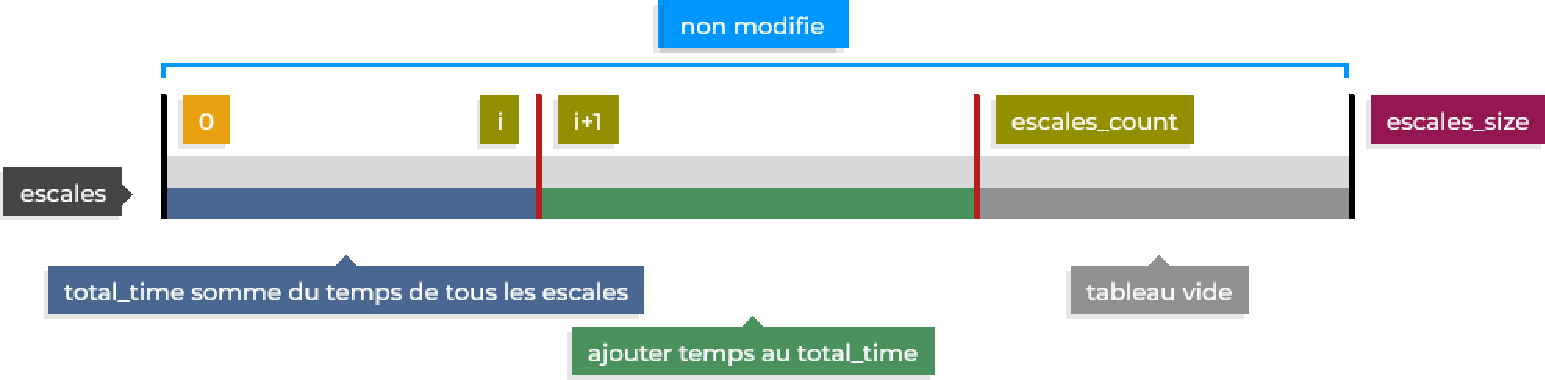
\includegraphics[width=1\textwidth]{invariant_time.pdf}
    \caption{Invariant graphique}
\end{figure}

\textbf{Invariant formel:} \\
    $escale = escale_0$ \\
    $\land$ \\
    $0 < i < escale\_count$ \\
    $\land$ \\
    $total\_time = \sum_{i=0}^{escale\_count-1} \texttt{get\_time}(escales[i])$


% !TEX root = ./main.tex
%%%%%%%%%%%%%%%%%%%%%%%%%%%%%%%%%%%%%%%%%%%%%%%%%%%%%%%%%%%%%%%%%%%%%%%%%%%%%%%%%%%%%%%%%%
% Justifiez, dans cette section, chacune de vos implémentations récursives à l'aide des  %
% 3 étapes vues au cours (cfr. Chap. 4)                                                  %
%%%%%%%%%%%%%%%%%%%%%%%%%%%%%%%%%%%%%%%%%%%%%%%%%%%%%%%%%%%%%%%%%%%%%%%%%%%%%%%%%%%%%%%%%%
\section{Implémentations Récursives}\label{recursivite}
%%%%%%%%%%%%%%%%%%%%%%%%%%%%%%%%%%%%%

Définition récursive:


course\_get\_escales\_count(course) = $
                \begin{cases}
                    return\ 0; & \text{if } course == NULL \\
                    return\ course\_get\_escales\_count(course->next) + 1; & \text{otherwise}
                \end{cases} $


course\_get\_stages\_count(course) = $
                \begin{cases}
                    return\ 0; & \text{if } course == NULL \\
                    return\ 0; & \text{if } course->next == NULL \\
                    return\ course\_get\_stages\_count(course->next) + 1; & \text{otherwise}
                \end{cases} $

course\_total\_time(course) = $
                \begin{cases}
                    return\ 0; & \text{if } course == NULL \\
                    return\ course\_total\_time(course->next) + escale\_get\_best\_time(course->escale); & \text{otherwise}
                \end{cases} $

course\_best\_time\_at(course, index) = $
                \begin{cases}
                    return\ escale\_get\_best\_time(course->escale); & \text{if } index == 0 \\
                    return\ course\_best\_time\_at(course->next, index - 1); & \text{otherwise}
                \end{cases} $

course\_append(course, escale) = $
                \begin{cases}
                    course = malloc(sizeof(Course)); \\
                    course->escale = escale; \\
                    course->next = NULL; \\
                    return\ course; & \text{if } course == NULL \\
                    \\
                    course->next = course_append(course->next, escale);\\
                    return\ course; & \text{otherwise}
                \end{cases} $

course\_pop(course) = $
                \begin{cases}
                    course = malloc(sizeof(Course)); \\
                    course->escale = escale; \\
                    course->next = NULL; \\
                    return\ course; & \text{if } course->next == NULL \\
                    \\
                    course->next = course_append(course->next, escale);\\
                    return\ course; & \text{otherwise}
                \end{cases} $

\[
\text{course\_append}(C, e) =
\begin{cases}
    \text{new}(e) & \text{if } C = \text{null} \\
    C \oplus \{\text{next} \mapsto \text{course\_append}(C.\text{next}, e)\} & \text{else}
\end{cases}
\]














% !TEX root = ./main.tex
%%%%%%%%%%%%%%%%%%%%%%%%%%%%%%%%%%%%%%%%%%%%%%%%%%%%%%%%%%%%%%%%%%%%%%%%%%%%%%%%%%%%%%%%%%
% Dans cette section, vous devez étudier complètement la complexité de votre code.       %
% Soyez le plus formel (i.e., mathématique) possible.                                    %
%%%%%%%%%%%%%%%%%%%%%%%%%%%%%%%%%%%%%%%%%%%%%%%%%%%%%%%%%%%%%%%%%%%%%%%%%%%%%%%%%%%%%%%%%%
\section{Complexité}\label{complexite}
%%%%%%%%%%%%%%%%%%%%

\subsection{Fonctions sur Escale}

\begin{itemize}
    \item escale\_create : $\mathcal{O}(1)$
    \item escale\_get\_name : $\mathcal{O}(1)$
    \item escale\_get\_x : $\mathcal{O}(1)$
    \item escale\_get\_y : $\mathcal{O}(1)$
    \item escale\_get\_best\_time : $\mathcal{O}(1)$
    \item escale\_set\_best\_time : $\mathcal{O}(1)$
    \item escale\_distance : $\mathcal{O}(1)$
    \item escale\_equal : $\mathcal{O}(1)$
\end{itemize}

\subsection{Opérations sur Course (tableau dynamique)}
Soit $n$ le nombre d'escales, $S$ la capacité du tableau.

\begin{align*}
&\texttt{course\_append} :
    \begin{cases}
        \mathcal{O}(1) & \text{(amorti)} \\
        \mathcal{O}(n) & \text{(réallocation)}
    \end{cases} \\
&\texttt{course\_pop} : \mathcal{O}(1) \\
&\texttt{course\_get\_escales\_count} : \mathcal{O}(1) \\
&\texttt{course\_total\_time} : \mathcal{O}(n) \\
&\texttt{course\_best\_time\_at}(i) : \mathcal{O}(1) \\
&\text{Espace mémoire} : \mathcal{O}(S),\ S \geq n
\end{align*}

\subsection{Opérations sur \texttt{Course} (liste chaînée)}

Soit $n$ le nombre d'escales.

\begin{align*}
&\texttt{course\_append} : \mathcal{O}(n) \\
&\texttt{course\_pop} : \mathcal{O}(n) \\
&\texttt{course\_get\_escales\_count} : \mathcal{O}(n) \\
&\texttt{course\_total\_time} : \mathcal{O}(n) \\
&\texttt{course\_best\_time\_at}(i) : \mathcal{O}(i) \\
&\texttt{course\_last} : \mathcal{O}(n) \\
&\text{Espace mémoire} : \mathcal{O}(n)
\end{align*}


% !TEX root = ./main.tex
%%%%%%%%%%%%%%%%%%%%%%%%%%%%%%%%%%%%%%%%%%%%%%%%%%%%%%%%%%%%%%%%%%%%%%%%%%%%%%%%%%%%%%%%%%
% Dans cette section, décrivez comment vous avez implémenté les différents tests         %
% unitaires                                                                              %
% Pensez à justifier vos choix.                                                          %
%%%%%%%%%%%%%%%%%%%%%%%%%%%%%%%%%%%%%%%%%%%%%%%%%%%%%%%%%%%%%%%%%%%%%%%%%%%%%%%%%%%%%%%%%%
\section{Tests Unitaires}\label{tests}
%%%%%%%%%%%%%%%%%%%%%%%%%


% !TEX root = ./main.tex
%%%%%%%%%%%%%%%%%%%%%%%%%%%%%%%%%%%%%%%%%%%%%%%%%%%%%%%%%%%%%%%%%%%%%%%%%%%%%%%%%%%%%%%%%%
% Rédigez ici la conclusion de votre rapport.                                            %
%%%%%%%%%%%%%%%%%%%%%%%%%%%%%%%%%%%%%%%%%%%%%%%%%%%%%%%%%%%%%%%%%%%%%%%%%%%%%%%%%%%%%%%%%%
\section{Conclusion}\label{conclusion}
%%%%%%%%%%%%%%%%%%%%%

C'est un cours difficile


%%%%%%%%%%%%%%%%%%%% FIN DE LA ZONE PROTÉGÉE %%%%%%%%%%%%%%%%%%%%

\end{document}
